%last updated in April 2002 by Antje Endemann

\documentclass[runningheads]{llncs}
%In order to omit page numbers and running heads
%please use the following line instead of the first command line:
%\documentclass{llncs}.
%Furthermore change the line \pagestyle{headings} to
%\pagestyle{empty}.

\usepackage[pdftex]{graphicx}
% declare the path(s) where your graphic files are
\graphicspath{{./figures/}}
% and their extensions so you won't have to specify these with
% every instance of \includegraphics
\DeclareGraphicsExtensions{.pdf}

\usepackage[cmex10]{amsmath}
\usepackage{mathrsfs}
\usepackage{amsfonts}
\usepackage{multirow}

\def\x{{\mathbf x}}
\def\L{{\cal L}}
\def\S{{\cal S}}
\def\N{{\cal N}}
\def\A{{\mathbf A}}
\def\B{{\mathbf B}}
\def\M{{\cal M}}

\input{psfig.sty}

\begin{document}

\pagestyle{headings}
%In order to omit page numbers and running heads
%please change this line to
%\pagestyle{empty}
%and change the first command line too, see above.

\mainmatter

\title{Feature evaluation for handwritten character recognition with regressive and generative Hidden Markov Models}

\titlerunning{Lecture Notes in Computer Science}

\maketitle

\begin{abstract}
Hidden Markov Models constitute an established approach often employed for offline handwritten character recognition in digitized documents. The current work aims at evaluating a number of procedures frequently used to define features in the character recognition literature, within a common Hidden Markov Model framework. By separating model and feature structure, this should give a more clear indication of the relative advantage of different families of visual features used for character classification. The effects of model topologies and data normalization are also studied over two different handwritten data-sets. The Hidden Markov Model framework is then used to generate images of handwritten characters, to give an accessible visual illustration of the power of different features.
\end{abstract}

\section{Introduction}
\label{sec:intro}
Transcription of digitized handwritten documents is an important task gaining lot of attention from the image processing and pattern recognition research community. Degradation of the documents over time, variation in writing styles, and inconsistent document background based on the medium, are but a few of the challenges encountered when working in this field in particular historical handwriting. One of the methods that has been successful in this area are the hidden Markov models (HMMs) \cite{Fink09}. Within natural-language processing, these models were used for speech recognition early on, and are good at handling discrete and continuous sequences of data. Since text is often written along one direction, handling text as a sequence of characters that can be explained with a language model fits well within the HMM paradigm.

%The process of training an HMM of \emph{first order} (i.e. current state depends only on the previous state) with a finite, discrete state space, depends on computing a matrix of \emph{state transition probabilities} denoted by $\A$, a vector of \emph{start probabilities} denoted by $\pi$, a matrix of state-specific \emph{emission probabilities} distributions denoted by $\B$.
% CN: I am more familiar with the terminology "emission probabilities"
The process of training an HMM with a finite, discrete state space, depends on computing a matrix of \emph{state transition probabilities} denoted by $\A$, a vector of \emph{start probabilities} denoted by $\pi$, a matrix of state-specific \emph{emission probabilities} distributions denoted by $\B$ which are computed by training relevant examples. In the current context, we consider the Baum-Welch and Bakis algorithms. The Baum-Welch algorithm is an Expectation-Maximization procedure that tries to answer question of determining the $(\pi, \A, \B)$ parameters which, help maximizing the HMM performance. However, there is an inherent directionality in Latin based text which is exploited in the \emph{left-right} topology using Bakis algorithm. Here the states move left to right but not the other way around. Further details on HMM implementation can be found in \cite{Rabi89}.
% CN NOTE TO SELF (mostly): BW does not necessarily assume a fully ergodic structure. Should
% go back to original Rabiner papers on this...

As HMMs are efficient at handling sequential information, images are often processed using a sliding window. The sliding window approach can be used at word or character level to identify words or characters respectively \cite{Fink09}. In the current approach the content within each window is used to extract features, which are then labeled. By concatenating labels of successive sliding windows, a string is formed corresponding to the original image. A HMM-bank, containing multiple disjoint HMMs is trained on the labeled training sequences. A query image is then classified based on a scoring mechanism over all the HMMs in the bank. The HMM in the bank that is trained on instances of a character giving the most favorable likelihood for the whole sequence of labels is selected as the classifier output. This setup provides an ideal testing environment to understand the strengths of different image features when used along with a sliding-window HMM. A Support Vector Machine (SVM) classifier is also trained on the features under study, in order to provide a benchmark for comparison (Fig. {\ref{fig:architecture}}(i)).

% CN: a baseline is a rather naïve comparison. I think this is more of a benchmark or reference, since
% CN: you mention later on that this model design it is one of the BEST classifiers for
% CN: digit-identification

%This paper is structured into six sections, including this introduction. Insight into the HMM architecture used in our character classification application is provided in the second section. The third section provides a description of the features used in the training. Data-sets used in evaluating the features and the evaluation methodology is described in the fourth section followed by results and conclusions, respectively.

\section{Architecture HMM Classifier}
\label{sec:HMM}
\begin{figure}[t]

\begin{minipage}[b]{1.0\linewidth}
  \centering
  \centerline{\includegraphics[width=13.0cm,height=5.0cm]{architecture}}
\end{minipage}
\caption{An overview of the experimental setup with individual process blocks}
\label{fig:architecture}
%
\end{figure}

In order to evaluate various features we have used identical pre-processing and classification procedures for all feature sets tested. As shown in Fig. {\ref{fig:architecture}} each image is converted to a gray-scale image rescaled to $100 \times 100$ pixels (Fig. {\ref{fig:architecture}}(a),(b)). Binarization is carried out if it is necessary to to compute specific feature such as background to foreground transitions. The image is
% CN: Should we say sliding window or simply window? Sliding, to me, could indicate some degree of overlap, even if it does not technically say so. I think it might be good to use the same phrase in the introduction and here, or at least clearly connect the more technical ``non-overlapping segmets'' to ``sliding windows''.
then divided into overlapping patches allowing for about 50\% overlap over adjacent windows (can be stripes favored by Marti-Bunke type features or patch based Fig. {\ref{fig:architecture}}(c),(d)). Features are then extracted on each patch independently. The features thus accumulated over the training data are then clustered using k-Means and a label is assigned to each patch as per the cluster to which it belongs. The experiments are repeated with and without whitening the feature vector to understand its behavior.
% CN: Last two sentences here could be clarified, and/or benefit from more detail. How is the clustering done? The clustering would not be a necessary component of an HMM and could matter a great deal for the results downstream.

In the current context HMMs are primarily used as classifiers of labeled sequences. In transcription of documents in Latin based script one is likely to encounter alphabetic letters in both upper and lower case, so an individual class for each character in each case is defined. This architecture leads to an HMM-bank with 52 individual HMMs, one for each letter in upper and lower case. Virtual beginning and end states are introduced, denoted by \textit{start} and \textit{end}, respectively. In case the feature extraction step produces $n$ segments there will be $n + 2$ states in the HMMs. These special beginning and end states are included to facilitate concatenation multiple training observation sequences to form one observation sequence on which individual HMM is trained. The classification of a query image is done by converting it to a query string using the labels obtained from the k-Means clustering. The query string is then passed to each character HMM in the bank and likelihood score is returned. A decision based on the maximum score returned from HMM-bank results in the classification of the query image to a letter.\\
% CN: "to a unique alphabet"??? letter?

%\subsection{HMM Architecture}
%\label{ssec:archi}
% In order to train an HMM a basic assumption on the topology of the state transitions should be made. In transcription of document on Latin based scripts the left-right topology is a natural choice \cite{Laan}. The initialization of the transition and emission matrices are done in such a way that the following properties are fulfilled:

%\begin{itemize}
% \item Beginning and end states \textit{start}, \textit{stop} will always emit the special symbols @ and \$ respectively.
% \item The  \textit{start} state will always transit to the first normal state.
% \item The \textit{end} state always transits back to \textit{start}.
% \item The forward transition from all other states is to a state that has not been visited since the last visit to \textit{start}.
% CN: IMPORTANT! Last item here says NO self-loops. Is that true or is it not? If we have self-loops, this should be slightly reworded.
%\end{itemize}

%With a proper ordering of states, this could be though of as a strictly upper-triangular matrix.

%\subsection{Initial Parameter Selection}
%\label{ssec:init}
%There are many ways to generate an initial model, some techniques consider random initialization strategies, which assigns the values in the transition and emission matrices to random values. In count-based initialization approaches, the emission matrix is assigned based on frequency of labels from the training examples, the transition matrix however is assigned with uniform probability from the current state to all reachable states. We have adopted the count based initialization for faster training of the HMMs \cite{Laan}. With an appropriate number of training iterations, we found classification accuracy of both random and count-based initialization to be similar.


\section{Feature Extraction}
\label{sec:feat}
In the following section we provide a brief description of seven different feature extraction methods. They have all found previous use in character recognition. Some of these are unique to character recognition using HMMs, while others are widely known as generic feature extraction methods in image analysis and computer vision.

\subsection{Naive Strip features}
\label{ssec:nsf}
Each image is binarized and then divided into vertical segments. Within each segment connected components are identified and three of the maximal components are picked based on the component length, $C_l$. These components are then identified as long, $\L$ if $C_l \ge n\cdot w_d$, short, $\S$ if $w_d \le C_l < n \cdot w_d$, or none, $\N$ if $ C_l < w_d$, where $w_d$ is the width of the segment and $n$ is a scale-factor. Each segment can thus be identified with a triplet formed by $\L,\S,\N$. There can be 10 combinations of these triplets and these form the class labels for this feature.
% CN: How do we end up with 10?
% CN: I find it a bit disconcerting that we first say that we always cluster, and then we don't.
This rather naive approach tries to identify the alphabetic letters based on edge patterns in a non-overlapping moving window over an image  \cite{Cheriet}.
%The dimensionality of the resulting feature is equal to the number of segments the image was divided into.
% CN: Since we said previously that we looked at each feature per window, the dimensionality is not equal to the number of segments. We should try to make a consistent presentation here. The dimensionality seems to be 1 (with 10 values?), or just possibly 3.



\subsection{Marti-Bunke features}
\label{ssec:mbf}
This is a nine-dimensional feature that is obtained for each vertical segment of the image. This feature captures rough shape, texture and span information of a character by computing some statistics and estimates over each segment. The shape information is based on computing the upper and lower contour position of the character in each segment, and the gradient of the upper and lower contours of the segment. The texture information is retained in the number of background-foreground transitions and by computing the number of foreground pixels between the upper and lower contour divided by the height of the contour. The character span is estimated by computing mean, the center of gravity and the second order moment of the segment \cite{MartiBunke02}. For efficient computation of these features binarized as well as gray-scale images are required. This feature is a compact representation of the shape information, but lacks a scale estimate that is required in differentiating the upper and lower case alphabet for instance in the case  of \emph{x, o, c} etc.

\subsection{Gabor features}
\label{ssec:gbf}
The feature is built by dividing the gray-scale image into a grid. A complex Gaussian kernel is built with varying sigma at different angles between the real and imaginary part of the kernel (the argument of a complex number) \cite{CCPBN10}. The mean of the absolute value of the convolution output is set as the threshold and the count of instances that have exceeded this threshold in each grid at each scale and orientation is cascaded to form the overall feature vector \cite{LKF05}. In the current framework it is forty-dimensional (5 scales $\times$ 8 orientations) feature per patch are the default parameter settings.

% CN: How does the gabor feature interact with the canonical windows, the splitting into which we claimed were common for all features? Are all patches mapping to the same window ordered as a single vector, and then subjected to clustering?

\subsection{Discrete Cosine Transform features}
\label{ssec:dctf}
Each patch is then subjected to a discrete cosine transform (DCT)  \cite{ANR74}. As most of the energy content of the image is contained in the low frequency, the coefficients are reordered by zig-zag scan in each patch. The most significant coefficients per patch can be picked up and cascaded to form the feature vector. In the default settings ten most significant coefficients are picked for each patch.

\subsection{Histogram of Oriented Gradients features}
\label{ssec:hog}
For each of the patch gradients are computed along various orientations \cite{DT05},\cite{FGMR09}. A histogram over the computed gradients in the given patch is cascade into a feature vector. In the current setup this is a 31-dimensional vector per patch.

\subsection{Pyramid Histogram Of visual Words features}
\label{ssec:phow}
This feature is a bag of dense Scale Invariant Feature Transform (SIFT) features at various scales \cite{Bosch07a}. This is a 512 dimensional feature vector due to the accumulation of 128 dimensional SIFT features at 4 scales.

\subsection{Local Binary Patterns features}
\label{ssec:lbp}
Within each selected path the center pixel is compared with every other pixel in a 3 $\times$ 3 neighborhood. Comparison between the pixels in encoded into a 8-dimensional vector of 0s and 1s depending on the gray scale value of the central pixel being higher or lower than the neighbor respectively. The vector can thus be a 128 dimensional but is quantized into 58 possible patterns thus resulting in 58 dimensional vector averaging over the patch. \cite{OPH94}.

% CN: Again, really try fo point out what is common, refer to the windows we claimed were common, and discuss how (and if) we cluster. Be consistent in specifying dimensionality with regards to either the full image, OR each patch/window, or at least specify dimensionality multiplied by factors that map to these quantities. In the Gabor dimensionality, I guess n_g could be decomposed into n_h and n_v (horizontal/vertical), where n_h is maybe the number of windows.

\section{Experiments}
All the experiments were conducted using two data sets as described below.
\label{sec:exp}
% -------------------------------------------------------------------------
\begin{figure}[t]

\begin{minipage}[b]{1.0\linewidth}
  \centering
  \centerline{\includegraphics[width=6.8cm,height=3.6cm]{data}}
%  \vspace{2.0cm}
%  \centerline{(a) Result 1}\medskip
\end{minipage}
\caption{Instances of 'a' in UniPenn(first row), NIST (second row)}
\label{fig:dataset}
%
\end{figure}

\subsection{Data-sets}
\label{ssec:data}
\subsubsection{UJIPenchar2}
The UJIPenchar2 dataset of online handwritten characters \cite{UJIPen} captures the stylus co-ordinates of 60 writers when writing two instances of each character in upper and lower case. This data-set has recorded information of 120 instances of each character as an (x,y)-coordinate trace of the pen. This on-line pen information is converted to offline images of characters using spline interpolation tracing the pen trajectory from captured coordinates. These images are subjected to  morphological erosion with a $3\times3$ cross structuring element to create characters of varying stroke width. Then a series of affine transformations are applied to the resulting images such as clockwise and counter-clockwise rotation about the vertical axis by 10 degrees, skewing the image in horizontal and vertical direction and adding noise along the edges of the character thus creating 3600 instances of each letter as shown in Fig.\ref{fig:dataset}.
% CN: Does this mean that the test dataset can include an affine transform of a letter from the hand
% CN: included in the training dataset. Have we done at least preliminary checks of leave-one-out
% CN: performance? (i.e. excluding all instances of one writer from the training set, and then testing
% CN: on that writer)

\subsubsection{NIST-19}
The NIST dataset consists of handwritten forms from 2100 different users provided with a form based handprint recognition system. About 1472 instances per lowercase character as shown in Fig.\ref{fig:dataset}, were extracted from these forms using the underlying recognition system \cite{NIST19}.

\subsection{Evaluation}
On each of the datasets a random sample of 1012 images are picked of which 512 are used for training and 500 images are used for testing. The results reported here are percentage of classification accuracy $\% accuracy = \frac{T_c}{N} \time 100$, where $T_c$ are images correctly labeled in the test set and $N$ total number of test images averaged over all the letters. 

The experiments can be broadly classified into two classes. First, a regressive evaluation of classification accuracy of the HMM classifier trained on each of the features described previously are benchmarked against SVM using a polynomial kernel of degree three. The focus has been on not only understanding the classification capability of the features, but also capture the parameter settings that are well suited for each method such as effect of whitening and k-Means clusters which directly influence the number of labels at each state in the HMMs.
% CN: HERE you mention that you do k-Means (and k-Means still has to be qualified).
These parameter settings are then used in the experiments where the HMMs are used as a generative models for characters in order to further understand the feature in capturing the variance in the handwriting over characters. The results from the generative model are useful in visually interpreting the performance of features and also the role of better resolution on performance of HMMs.

% CN: See previous comment on how to sample a structured random dataset. This could be even more true for the SVM method, which might overfit due to artificially high similarity between training and sample.

\label{ssec:eval}
\subsection{Regression Tests}
\subsubsection{Number of kMeans clusters:} In state of the art HMMs for handwriting transcription labeling the feature vector is done through training Gaussian Mixture models. The features are used to train a mixture model with 4 distributions. This model is in turn used to initialize and train a mixture with 8 distributions and this procedure is repeated successively to obtain a model with either 16 or 32 distributions \cite{Young}. In a similar spirit we have clustered the features using kMeans with k=5,10,...40 and found that going beyond k=20 does not yield any significant improvement in classification accuracy but makes the HMM training slower due to more labels. Effect of moving from k=10 to k=20 is shown in Fig. {{\ref{fig:kmeans}}. For all the experiments that follow k=20 during the k-Means clustering step.
\begin{figure}[t]
\begin{minipage}[b]{1.0\linewidth}
  \centering
  \centerline{\includegraphics[width=10.0cm,height=5.0cm]{bar}}
\end{minipage}
\caption{Comparison of classification accuracy percentage of HMM classifier wiht k-Means Clustering with k=10 and k=20}
\label{fig:kmeans}
\end{figure}

%The overall evaluation is calculated as a percentage of images classified correctly in the testing images as shown in Table\ref{table01}. The results provided here are based on manually tuning the parameters of each feature to obtain the best performance within reasonable computation time over several experiments. Effect of increasing the number of k-Means clusters shown in Fig.\ref{fig:kmeans}. It has been observed that increasing the number of k-Means centroids beyond twenty does not effect the results as the most of the cluster have very few data points.
% CN: What number is "very few"? Are some clusters heavily populated? Considering the number of unique
% CN: training samples, there seems like there could be far more. The clustering is done over all
% CN: feature vectors found in the full dataset, right?
\subsubsection{Topology and whitening of data:} Two topologies tested in these experiments are the Ergodic and the Bakis topologies. The classification accuracy for these topologies are mostly similar. The results with and without of data whitening on the two HMMS topologies are available in Table{\ref{table01}}. The results from HMM classifier are compared with SVM with a polynomial kernel of degree three which is one of the top performing classifier on NIST digits dataset \cite{LeCun98} with the entire image is used as input. This result is reported in Table {\ref{table01}}. However, to make the comparison more fair, we also feed the SVM with feature data, in Table {\ref{table02}}.
\begin{table*}[!t]
\caption{Classification accuracy percentages for HMM and SVM Classifiers}
\label{table01}
\centering
\begin{tabular}[t]{|c|c|c|c|c|c|}
\hline
\multicolumn{1}{ |c| }{\multirow{2}{*}{Feature} } &
\multicolumn{2}{ |c| }{Ergodic} & \multicolumn{2}{ |c| }{Bakis} &
\multicolumn{1}{ |c| }{\multirow{2}{*}{Whitened} } \\ \cline{2-5} &
\multicolumn{1}{ |c| }{UniPenn} & NIST & UniPenn & NIST & \\ \hline
Naive-Strip & 12.9 & 26.13 &  12.92 & 25.49 & \multirow{4}{*}{Yes}\\ \cline{1-5}
Marti-Bunke & 43.36 & 66.68 & 43.46 & 67.09 & \\ \cline{1-5}
Gabor & 52.24 & 70.48 & 52.24 & 70.5 & \\ \cline{1-5}
DCT & 59.37 & 72.82 & 60.89 & 73.76 & \\ \cline{1-5}
HOG & 63.36 & 77.68 & 64.58 & 76.82 & \\ \cline{1-5}
PHOW & 52.24 & 70.48 & 48.38 & 68.68 & \\ \cline{1-5}
LBP & 42.37 & 65.82 & 41.56 & 65.76 & \\ \hline \hline
Naive-Strip & 12.9 & 26.13 & 12.92 & 25.49 & \multirow{4}{*}{No}\\ \cline{1-5}
Marti-Bunke & 37.68 & 65.47 & 38.2 & 66.0 & \\ \cline{1-5}
Gabor & 54.24 & 71.99 & 54.23 & 71.93 & \\ \cline{1-5}
DCT & 61.43 & 74.18 & 61.09 & 74.0 & \\ \cline{1-5}
HOG & 65.16 & 79.66 & 66.48 & 77.32 & \\ \cline{1-5}
PHOW & 55.94 & 72.38 & 53.03 & 71.86 & \\ \cline{1-5}
LBP & 45.30 & 69.22 & 44.16 & 67.76 & \\ \hline \hline
SVM poly. deg. 3 & 75.75 & 85.63 & - & - & \multirow{1}{*}{-}\\ \cline{1-6}

\end{tabular}
\end{table*}

\subsubsection{Sliding windows:}
It is a common practice in word and character HMMs to apply the sliding window from left to right and feed the HMM with features from thin overlapping image stripes. In this paper we extend this paradigm, also sweeping top-down and testing square shaped patches, and investigate whether the performance of the HMMs is improved. The size and step length of the sliding window in these cases are calculated such that length of the label sequence generated per image in both the methods are almost same, thus no bias in introduced in the HMM training. Table{\ref{table02}} shows the comparison between Marti-Bunke and DCT. As the dimensionality of these features are nine and ten respectively, they are comparable. 
% CN: Added sentence above.

\begin{table*}[!h]
\caption{Comparison of features for patch vs strip based sliding window approach}
\label{table02}
\centering
\begin{tabular}[t]{|c|c|c|}
\hline
Feature & UniPenn & NIST \\ \hline
HMM + MB + Strip & 43.46 & 67.09 \\ \hline
HMM + MB + Patch & 45.90 & 75.83 \\ \hline
HMM + DCT + Strip & 44.77 & 67.85 \\ \hline
HMM + DCT + Patch & 59.79 & 76.09 \\ \hline \hline
SVM + MB + Strip & 59.56 & 82.23 \\ \hline
SVM + MB + Patch & 65.79 & 85.67 \\ \hline
SVM + DCT + Strip & 58.54 & 84.34 \\ \hline
SVM + DCT + Patch & 60.32 & 85.0 \\ \hline
\end{tabular}
\end{table*}

\subsection{Generative Tests}
In the final experiments, we use the trained HMMs as generative models instead of classifiers. The results are synthesized instances of characters, which gives a glimpse of what a given HMM model is able to capture. It also enable us to make a qualitative comparison between features through the analysis of the emission matrix ($\B$). The most probable state transitions are generated from the transition matrix ($\A$) and the label at each state is generated from the emission matrix ($\B$). The image corresponding to the label are generated from the k-Means cluster center of that label. This approach has two benefits. Firstly, it provides a qualitative way to visualize the results by showing the extent of variation in the writing of each character as captured by the features. Fig. {\ref{fig:chars}} helps in comparing the letters generated with strip and patch mode, by comparing top and middle rows, and also features from Marti-Bunke and DCT features by comparing the middle and bottom rows.

% CN: Considering that we want to evaluate the feature space, would it make sense to re-render the examples in Fig 1. with a simple auto-encoding, i.e. go from image to feature space and go back again using the same method as here. (I.e. illustrate the image corruption, as seen by the human eye, by just doing the feature encoding, no classification or model.) Making a generative example from the SVM would also make sense to put the generative examples here in context, but I am more keen on the auto-encoder idea.

\begin{figure}[!h]
\begin{minipage}[b]{1.0\linewidth}
  \centering
  \centerline{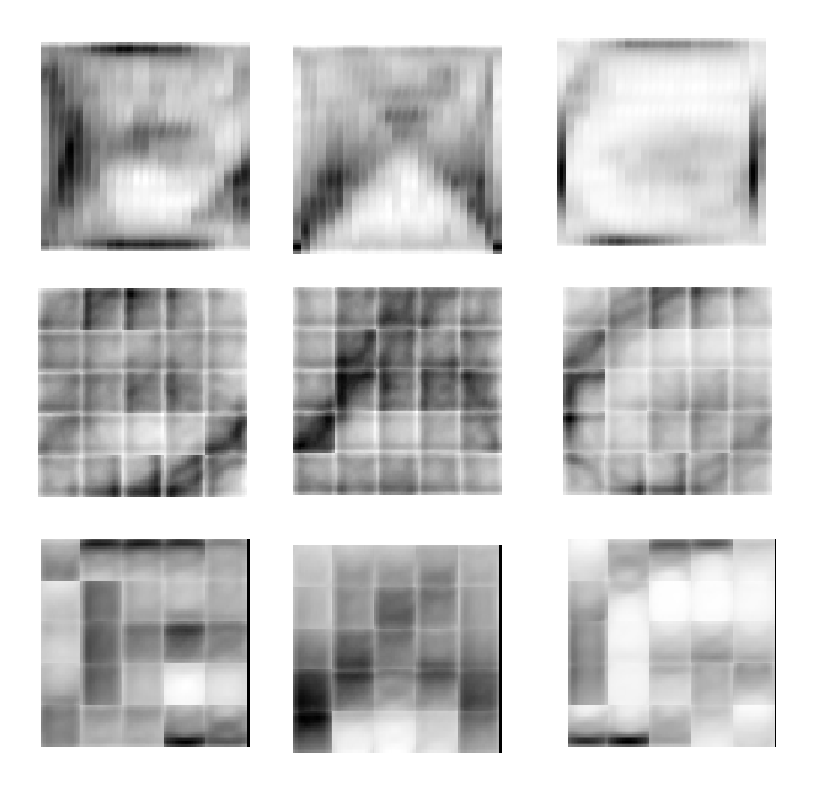
\includegraphics[width=5.0cm,height=5.0cm]{char}}
\end{minipage}
\caption{Character instances of B,A,G from HMMs. top row: DCT+strip, middle row: DCT+patch, bottom row: MB+patch}
\label{fig:chars}
\end{figure}

Secondly, a the generative experiments helps to analyze the learning transfered to HMMs through the features. By construction, for an HMM with with $N_s$ states its transition matrix ($\A$) is square and diagonal dominant as we are forcing a inherent directionality through the way the image of the character is swept. The variation in the various handwritten characters are captured in the emission matrix ($\B$), which is a rectangular matrix of size $N_s \times N_l$, where $N_l$ are number of emission labels at each state. In order to capture this variation efficiently, matrix $\B$ has to be of full rank. By performing a low rank approximation of $\B$, we can determine which feature is efficient. In the current experiment $N_s$ = 25, $N_l$ = 20. For an efficient feature, the rank for the low rank approximation of $\B$ needs to be as high as possible, i.e as close to 20 as possible. Fig. {\ref{fig:rank}} shows these results in parallel coordinates \cite{Moustafa11} representation of the rank for Marti-Bunke and DCT features respectively to limit the width of the graph only the result for HMMs trained for upper case letters is provided.

% CN: I really don't understand this argument. I can see the reduced rank representation as relevant,
% CN: but I am not sure if you mean variance or variation, or in what sense.

\begin{figure}[!t]
\begin{minipage}[b]{1.0\linewidth}
  \centering
  \centerline{\includegraphics[width=10.0cm,height=6.0cm]{rank}}
\end{minipage}
\caption{Reduced rank of emission matrices over various character HMMs}
\label{fig:rank}
\end{figure}

% CN: Remove lines. And/or consider sorting the alphabet by character complexity. (Add rank for all models and then sort characters accordingly, i.e. Q very early and V, C rather late). Adjust vertical axis to start at 0.
% CN: It could make sense to also look at reduced ranks of B'.

\section{Conclusions}
\label{sec:conc}
% CN: Could we show to representative transition matrices (with logged probabilities) indicating that 
% CN: the effective structure is indeed similar. The ergodic matrix might need to be "sorted" to produce
% CN: a similary band-like structure.

% CN: Did you verify the produced log-likelihoods after training compared to log-likelihood after initing?
% CN: How do you handle zero counts in the count-init?

%The HMMs performance of the ergodic and left-right topologies are almost identical over all the features. The Marti-Bunke performs well when increasing the number of segments into which the image is divided into but suffers from performance issues when the sequence length get longer. Gabor feature outperform other features primarily due to the effectively handling the scaling that occurs over upper and lower case characters such as \emph{c,k,o,p,x}. The features that are able to encode the scaling information such as histogram of oriented gradients (HOG) and DCT are able to out perform the other features such as Marti-Bunke and local binary patterns. The DCT feature is effective in encoding information in the lower dimension with performance at par with HOG which are three time more in dimensionality. The results show a clear indication that performance of HMMs can be improved by moving over to a patch based sliding window approach.


The HMMs performance of the ergodic and left-right topologies are almost identical over all the features. The Marti-Bunke features performs well when increasing the number of segments that divides the image. However, Marti-Bunke features suffers from performance issues when the sequence length get longer. Features that are able to encode the scaling information, such as HoG, Gabor and DCT, are able to outperform the other features such as Marti-Bunke and local binary patterns. This is particularly due to effectively handling the scaling that occurs over upper and lower case characters such as c,k,o,p,x. The best performing feature extration appears to be HoG. DCT has only slightly worse performance than HoG, but is more compact (1/3 of the dimensionality). The results indicate that performance of character recognition HMMs could be improved, by moving from a strip based sliding window approach to a patch based. Finally, The SVM classifier, which processes all feature values in parallel rather than as a sequence, consistently beats HMM. This indicates that HMMs may suffer from their inherently one-dimensional data processing, in this particular application. 

%\section{Acknowledgement}
%\label{sec:ackno}
%The authors would like to thank Alicia Fornes and Computer Vision Center at Universitat Autonoma de Barcelona for their help in extracting the character images from the NIST data-set. The research is funded by "Vetenskapsr\r{a}det grant 2012-5743" and the "q2b -- From Quill 2 Bytes initiative at Uppsala University".

\nocite{bal:cha:gra:pae}
\bibliographystyle{splncs}
\bibliography{isvc}

\end{document}
